
\documentclass[a4paper, 11pt, oneside]{article}

\usepackage[utf8]{inputenc}
\usepackage[T1]{fontenc}
\usepackage[french]{babel}
\usepackage{array}
\usepackage{shortvrb}
\usepackage{listings}
\usepackage[fleqn]{amsmath}
\frenchbsetup{StandardLists=true} % à inclure si on utilise \usepackage[french]{babel}
\usepackage{amsfonts}
\usepackage{fullpage}
\usepackage{enumerate}
\usepackage{graphicx}             % import, scale, and rotate graphics
\usepackage{subfigure}            % group figures
\usepackage{enumitem}
\usepackage{amssymb}
\usepackage{alltt}
\usepackage{url}
\usepackage{indentfirst}
\usepackage{eurosym}
\usepackage{listings}
\usepackage{color}
\usepackage[table,xcdraw,dvipsnames]{xcolor}
\usepackage{wrapfig}
\usepackage{minitoc}
\usepackage{clrscode3e}



% Change le nom par défaut des listing
\renewcommand{\lstlistingname}{Extrait de Code}

% Change la police des titres pour convenir à votre seul lecteur
\usepackage{sectsty}
\allsectionsfont{\sffamily\mdseries\upshape} 
% Idem pour la table des matière.
\usepackage[nottoc,notlof,notlot]{tocbibind} 
\usepackage[titles,subfigure]{tocloft} 
\renewcommand{\cftsecfont}{\rmfamily\mdseries\upshape}
\renewcommand{\cftsecpagefont}{\rmfamily\mdseries\upshape} 

\definecolor{mygray}{rgb}{0.5,0.5,0.5}
\newcommand{\coms}[1]{\textcolor{MidnightBlue}{#1}}

\lstset{
    language=C, % Utilisation du langage C
    commentstyle={\color{MidnightBlue}}, % Couleur des commentaires
    frame=single, % Entoure le code d'un joli cadre
    rulecolor=\color{black}, % Couleur de la ligne qui forme le cadre
    stringstyle=\color{RawSienna}, % Couleur des chaines de caractères
    numbers=left, % Ajoute une numérotation des lignes à gauche
    numbersep=5pt, % Distance entre les numérots de lignes et le code
    numberstyle=\tiny\color{mygray}, % Couleur des numéros de lignes
    basicstyle=\tt\footnotesize, 
    tabsize=3, % Largeur des tabulations par défaut
    keywordstyle=\tt\bf\footnotesize\color{Sepia}, % Style des mots-clés
    extendedchars=true, 
    captionpos=b, % sets the caption-position to bottom
    texcl=true, % Commentaires sur une ligne interprétés en Latex
    showstringspaces=false, % Ne montre pas les espace dans les chaines de caractères
    escapeinside={(>}{<)}, % Permet de mettre du latex entre des <( et )>.
    inputencoding=utf8,
    literate=
  {á}{{\'a}}1 {é}{{\'e}}1 {í}{{\'i}}1 {ó}{{\'o}}1 {ú}{{\'u}}1
  {Á}{{\'A}}1 {É}{{\'E}}1 {Í}{{\'I}}1 {Ó}{{\'O}}1 {Ú}{{\'U}}1
  {à}{{\`a}}1 {è}{{\`e}}1 {ì}{{\`i}}1 {ò}{{\`o}}1 {ù}{{\`u}}1
  {À}{{\`A}}1 {È}{{\`E}}1 {Ì}{{\`I}}1 {Ò}{{\`O}}1 {Ù}{{\`U}}1
  {ä}{{\"a}}1 {ë}{{\"e}}1 {ï}{{\"i}}1 {ö}{{\"o}}1 {ü}{{\"u}}1
  {Ä}{{\"A}}1 {Ë}{{\"E}}1 {Ï}{{\"I}}1 {Ö}{{\"O}}1 {Ü}{{\"U}}1
  {â}{{\^a}}1 {ê}{{\^e}}1 {î}{{\^i}}1 {ô}{{\^o}}1 {û}{{\^u}}1
  {Â}{{\^A}}1 {Ê}{{\^E}}1 {Î}{{\^I}}1 {Ô}{{\^O}}1 {Û}{{\^U}}1
  {œ}{{\oe}}1 {Œ}{{\OE}}1 {æ}{{\ae}}1 {Æ}{{\AE}}1 {ß}{{\ss}}1
  {ű}{{\H{u}}}1 {Ű}{{\H{U}}}1 {ő}{{\H{o}}}1 {Ő}{{\H{O}}}1
  {ç}{{\c c}}1 {Ç}{{\c C}}1 {ø}{{\o}}1 {å}{{\r a}}1 {Å}{{\r A}}1
  {€}{{\euro}}1 {£}{{\pounds}}1 {«}{{\guillemotleft}}1
  {»}{{\guillemotright}}1 {ñ}{{\~n}}1 {Ñ}{{\~N}}1 {¿}{{?`}}1
}
\newcommand{\tablemat}{~}

%%%%%%%%%%%%%%%%% TITRE %%%%%%%%%%%%%%%%
% Complétez et décommentez les définitions de macros suivantes :
 \newcommand{\intitule}{Projet 1: Algorithme de tri}
 \newcommand{\PrenomUN}{Julien}
 \newcommand{\NomUN}{Gustin}
 \newcommand{\PrenomDEUX}{Mathias}
 \newcommand{\NomDEUX}{Carlisi}
 %Décommentez ceci si vous voulez une table des matières :
 \renewcommand{\tablemat}{\tableofcontents}

%%%%%%%% ZONE PROTÉGÉE : MODIFIEZ UNE DES DIX PROCHAINES %%%%%%%%
%%%%%%%%            LIGNES POUR PERDRE 2 PTS.            %%%%%%%%
\title{INFO2050: \intitule}
\author{\PrenomUN~\textsc{\NomUN}, \PrenomDEUX~\textsc{\NomDEUX}}
\date{}
\begin{document}
\maketitle
\newpage
%%%%%%%%%%%%%%%%%%%% FIN DE LA ZONE PROTÉGÉE %%%%%%%%%%%%%%%%%%%%

%%%%%%%%%%%%%%%% RAPPORT %%%%%%%%%%%%%%%
% Écrivez votre rapport ci-dessous.

	\section{Analyse théorique}
	\subsection{Invariant}
	\begin{itemize}[label=$\square$]

\item

	\noindent $\{P\} \gets$ "$A$ est un tableau d'entiers de taille $\attrib{A}{length}"$\\
	  $\{Q\} \gets$ "Le tableau $A$ est trié"\\ 
	$\{I\} \gets$ "Le sous tableau 
$A[1..i]$ contient les $i$ premiers éléments de $A$ triés, le sous tableau \indent \indent $A[j..A.length]$ est la partie du tableau de $A$ qui n'est pas encore triée"

\item $\{P\} i = 1$ $\&\&$ $j = 2 \{I\}$
\\ $\{I\}$  $\exists i,j,$ $1 \leq i < j \leq \attrib{A}{length},$  $A[1..i],$ $\forall k,$ $1 \leq k < i, A[k] \leq A[k+1]$ \\
\indent Fonction de terminaison : $f \gets \attrib{A}{length}-j +1$
\\ $\{Q\} = \forall k,$ $1 \leq k < \attrib{A}{length},$ $A[k] \leq A[k+1]$ $\&\&$ $j=\attrib{A}{length}+1$

\end{itemize}

	\subsection{PseudoCode}
	\label{PseudoCode}
	
	\begin{codebox}
\Procname{$\proc{New-Sort}(A)$}
\li $i \gets 1$

\li \For $j \gets 2$ \To $\attrib{A}{length}$ \color{Gray} //Parcours le tableau dans son entièreté
\Do

\li \While $A[j] \leq A[j+1]$ and $j < \attrib{A}{length}$
\li \Do
$j \gets j + 1$  \color{Gray} //Permet de trouver le prochain indice 'j' du tableau dont la valeur est triée
\End
\li $\proc{Merge}(A, 1, i, j)$  \color{Gray} //Fusionne deux sous tableaux triés A[1..i] et A[i+1..j]

\li $i \gets j$
\End
\end{codebox}

\subsection{Complexité}
La complexité en temps, dans le meilleur des cas, est $\Theta(n)$ ( si le tableau est pré-trié par ordre croissant ) et dans le pire des cas $\Theta(n^{2})$ ( si le tableau est pré-trié dans un ordre décroissant ) , où 'n' est la taille du tableau ( array ). En effet, si les valeurs sont triées par ordre croissant, nous itérons la boucle principale qu'une seule fois ainsi \textit{Merge} ( d'une complexité de $O(n)$ ) est appelé lui aussi une seule fois, au contraire si  les valeurs sont triées par ordre décroissant \textit{Merge} sera appelé 'n' fois parce que il n'existera aucun sous tableau trié, de taille plus grand que un, ainsi la boucle principale itéra 'n' fois.   \\ 
\textbf{Preuve :}\\ $T(n) \leq \sum_{i = 1}^{n} i$ \\ \indent Puisque \indent$\sum_{i = 1}^{n} i = \frac{n(n+1)}{2} \\ \indent$ On obtient $T(n) \leq \frac{n(n+1)}{2}$ \\
\indent ainsi nous obtenons $T(n) = O(n^{2})$ puisque nous bornons supérieurement

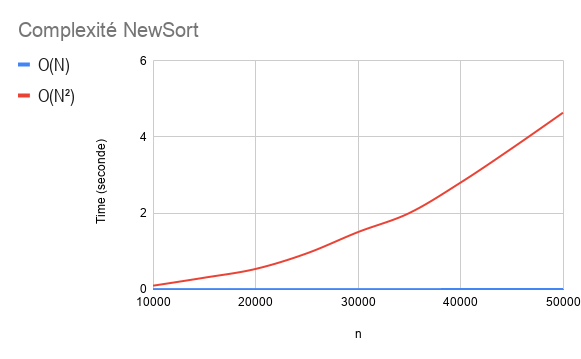
\includegraphics[scale=0.6]{graphique.png} \\
( Graphique testé avec des valeurs réelles, où O(n) correspond à un tableau pré-trié et O(n$^{2}$), pré-trié dans un ordre décroissant ) 


\subsection{Stabilité ?}
\textbf{NewSort}
 est un tri stable en effet, grâce a "\textit{$A[j]\leq A[j+1]$}"
	\footnote{\begin{codebox}
	\While $A[j] \leq A[j+1]$ and $j < \attrib{A}{length}$
voir PseudoCode~\ref{PseudoCode}
\End
\end{codebox} }
, les valeurs égales n'interchangent pas de place et sont considérées comme déjà triées, de plus vu que la fonction "\textit{Merge}" est stable. Donc, nous pouvons en conclure que \textbf{NewSort} est lui aussi stable. 


\subsection{Complexité au pire des cas}
Pour un tableau de taille 'n' constitué de $k(\leq n$) blocs pré-triés de taille identique nous avons une complexité ( au pire des cas ) de $\Theta(k \cdot n)$, en effet, si k = n nous avons une complexité de $\Theta(n^{2})$ et d'un autre coté si k = 1 nous avons $\Theta(n)$, respectivement nous avons bien le meilleur et le pire des cas décrit ci-dessus. Cela vient du fait que "\textit{Merge}" a une complexité de $O(n)$ qui est appelée au maximum \footnote{Deux blocs pré-trié différents peuvent très bien être trié entre eux ainsi ne forme qu'un et même seul bloc trié} 'k' fois vu que la boucle\footnote{\begin{codebox}
\li \While $A[j] \leq A[j+1]$ and $j < \attrib{A}{length}$
\li \Do
$j \gets j + 1$

\End
\end{codebox} }
secondaire permet de trouver l'indice du tableau auquel sa valeur à l'indice suivant est plus petit. Ainsi nous savons bien que dans le pire des cas \textit{Merge} est appelé 'k' fois. \\ \\
\textbf{Preuve :}
$\sum_{i = 1}^{k} i \cdot \frac{n}{k}$ $<=>$ $\frac{n}{k}\sum_{i = 1}^{k} i$ \\ 
\indent Puisque \indent$\sum_{i = 1}^{k} i = \frac{k(k+1)}{2}$ \\
\indent Nous avons : \indent $\frac{n}{k} \cdot \frac{k(k+1)}{2}$ $<=>$ $ \frac{n(k+1)}{2}$ \\ Nous bornons $T(n)$ et ainsi $T(n) = O(n \cdot k)$

\newpage

\section{Analyse expérimentale}
\subsection{Temps d'exécution sur des tableaux aléatoires}

\begin{table}[htb]
\begin{tabular}{cccccc}
\hline

n   & InsertionSort & QuickSort & HeapSort & MergeSort & NewSort \\ \hline
$10^{1}$ & 0,000015      & 0,000005  & 0,000006         & 0,000009          & 0,000005        \\
$10^{2}$ & 0,000052      & 0,000035  & 0,000061         & 0,000054          & 0,000090        \\
$10^{3}$ & 0,001055      & 0,000225  & 0,000959         & 0,000297          & 0,001841        \\
$10^{4}$ & 0,060314      & 0,003429  & 0,003847         & 0,002229          & 0,112815        \\
$10^{5}$ & 7,216459      & 0.036962  & 0,032527         & 0,017463           & 10,771157        \\
$10^{6}$ & 768,522644    & 2.639571  & 0,353273         & 0,179450          & 1429,154037
        
\end{tabular}
\end{table}


L'\textbf{InsertionSort} et le \textbf{NewSort} sont les tris les plus lents des cinq, en effet avec leurs complexités moyennes de $\Theta(n^{2})$, ces tris prennent un temps quadratique pour un tableau de taille 'n', cette complexité "élevée" découle du fait que, contrairement aux QuickSort, MergeSort ou HeapSort, ces tris requièrent de parcourir le tableau plusieurs fois afin d'y insérer une valeur à sa bonne place que ce soit par fusion ou insertion. 
\\ \\
\indent L'algorithme qui suit, \textbf{QuickSort} est de type "diviser pour régner" ( découper le problème initial en sous problèmes, résoudre ceux ci permet de résoudre le problème initial ), sa complexité moyenne est $\Theta(n$ $log$ $n$), cependant, sa lenteur  comparé à \textbf{MergeSort} et \textbf{HeapSort} est dû, aux pires de ses cas, avoir des valeurs triées par ordre croissant ou décroissant, le mène à avoir une complexité quadratique. Il procède ainsi par une méthode qui s'appelle "partition" et qui consiste à choisir un pivot que nous plaçons à la fin du sous tableau. Les éléments inférieurs à celui-ci sont insérés au début de ce sous tableau, ensuite ce pivot est placé à la fin des éléments déplacés, cette méthode permet de trier le tableau rapidement, cependant, si le tableau est déjà trié en entrée, ce tri n'est pas vraiment efficace.\\ 

Les deux prochains algorithmes, \textbf{HeapSort} et \textbf{MergeSort}, sont tous deux extrêmement rapides avec une complexité, que ce soit dans le pire ou le meilleur des cas de $\Theta(n$ $log$ $n$),  qui est asymptotiquement optimale. Le \textbf{MergeSort} est de type "diviser pour régner", cet algorithme fonctionne par le principe que, à partir de deux tableaux triés, nous pouvons former un tableau trié, ainsi par récursivité, nous créons des sous-tableaux de plus en plus petits jusqu'à ce que le tableau ne contienne plus qu'un seul élément et par la remontée récursive, nous fusionnons ces tableaux qui deviennent de plus en plus grands à chaque remontée jusqu'à ce que le tableau soit complètement trié.\\ Le \textbf{HeapSort} fonctionne par arbre binaire. ( L'absence de "pire cas" le rend "puissant" cependant dans des cas où la plage de nombres est plus élevées \textbf{QuickSort} est souvent préféré. ) \\
Ce qui crée la légère différence en temps entre ces deux tris est la stabilité. En effet, le HeapSort ne préserve pas nécessairement l’ordre des éléments à valeurs identiques contrairement au MergeSort qui gagne ainsi en rapidité.

\begin{table}[htb]
\begin{tabular}{cccccc}
\hline

Cas   & InsertionSort & QuickSort & HeapSort & MergeSort & NewSort \\ \hline
Meilleur & $\Theta(n)$      & $\Theta(n$ $log$ $n)$   & $\Theta(n$ $log$ $n)$        & $\Theta(n$ $log$ $n)$          & $\Theta(n)$        \\
Pire & $\Theta(n^{2})$     & $\Theta(n^{2})$  & $\Theta(n$ $log$ $n)$         & $\Theta(n$ $log$ $n)$ & $\Theta(n^{2})$       \\
Moyen & $\Theta(n^{2})$      & $\Theta(n$ $log$ $n)$  & $\Theta(n$ $log$ $n)$         & $\Theta(n$ $log$ $n)$         & $\Theta(n^{2})$        \\
Stable & Oui      & Non  & Non         & Oui          & Oui        \\
  
\end{tabular}
\end{table}

\section{Temps d'exécution sur des tableaux de blocs pré-triés}
\begin{table}[htb]
\begin{tabular}{llllll}
\hline
k    & InsertionSort & QuickSort & HeapSort & MergeSort & NewSort \\ \hline
1    & 0,000060              & 0,065099          & 0,002262         & 0,001146          & 0,000132        \\
20   & 0,014462              & 0,005105          & 0,002415         & 0,001470          & 0,000974        \\
100  & 0,015836              & 0,001485          & 0,001888      & 0,001702          & 0,002533        \\
500  & 0,01761              & 0,001638          & 0,001644         & 0,001810          & 0,006723        \\
1000 & 0,015769              & 0,001626          & 0,001752         & 0,001876          & 0,013732        \\
5000 & 0,030251              & 0,047346          & 0,002043         & 0,001124          & 0,058827       
\end{tabular}
\end{table}
Nous pouvons voir que pour un tableau pré-trié ( k = 1 ) \textbf{InsertionSort} et le \textbf{NewSort} sont les plus rapides. En effet, pour ces deux tris, un tableau pré-trié est leur meilleur cas, cependant en pratique ce sont les plus lents: avoir un tableau déjà trié en entrée est quelque chose de très très rare et inutile, et en comparant les valeurs de ces deux tris avec les trois autres nous remarquons que pour des cas plus probables ils sont moins efficaces... \\ \\
Le \textbf{QuickSort} est un algorithme très efficace si l'intervalle de rapport est plus élevé en effet vu que ce tri n'est pas stable avoir plusieurs valeurs les mêmes les unes à cotés des autres lui complique la tâche. De plus ses pires cas sont d'avoir comme pivot soit la valeur la plus petite soit la plus grande, autrement dit avoir un tableau trié par ordre croissant ou décroissant c'est pour cela que le quicksort atteint son efficacité maximale entre 'k' = 100 et 'k' = 1000 ( plus rapide que les 4 autres ), et au contraire est très peu efficace en 'k' = 1 ou 5000\\
\\
Le \textbf{HeapSort} et \textbf{MergeSort} sont tout les deux très rapides et constants, c'est ce qui constitue leur force, ils n'ont pas de meilleur ou pire cas. Cependant vu que le HeapSort n'est pas stable, pour un tableau qui contient des répétitions il est préférable de choisir le \textbf{MergeSort}.
\\ \\
En bref, \textsc{est-ce que le \textbf{NewSort} a un réel intérêt ?} \\ Pour un tableau de taille assez petit ( plus petit que $10^{3}$ ) avec des blocs pré-triés en amont, ce tri peut avoir un intérêt. Cependant en situation réelle il sera préférable de se diriger vers le QuickSort ou le MergeSort. 
 
\end{document}